\section{Details of the Real-World Setup}
\label{as:s2r}

\paragraph{Scene.} Our real-world experiments take place in a mockup studio-apartment in our lab that includes a bedroom, living room, and dining area. 
This real-world scene was modeled with a digital counterpart in simulation for \benchmark: the \texttt{mockup\_apt} scene. Fig.~\ref{fig:sim2real_setup} depicts both real and digital twin side-by-side. The digital model has been created by first, scanning the real-world apartment using a phone and commercial software~\cite{scaniverse}, then, replacing and projecting the texture of walls, floors, and ceilings, and finally, replacing the existing objects with 3D models from our \dataset. This process should minimize the effect caused by differences between the real world and the 3D model. The simulated and the real robot use the same 2D map of the scene for localization. In this way, 2D locations in the real world correspond to the same 2D locations in simulation. 

\paragraph{Robot platform.} We use in our experiments a Tiago++ model from PAL Robotics, with an omnidirectional base, two 7-degrees-of-freedom arms with parallel-yaw grippers, a 1-degree-of-freedom prismatic torso, two SICK LiDAR sensors (back and front of the base), and an ASUS Xtion RGB-D camera mounted on the robot's head, which can be controlled in yaw and pitch.
All sensors and actuators are connected through the Robot Operating System, ROS~\cite{quigley2009ros}. The code runs on a laptop with an Nvidia GTX 1070 that sends the commands to the onboard robot computer to be executed.

\paragraph{Action primitives on the real robot.} We implemented a version of the action primitives \texttt{navigate}, \texttt{pick} and \texttt{place} on the real robot similar to their implementation in \simulator. For navigation, we use a 2D sampling-based motion planner on the 2D map we use for localization and that has been created from the 3D model of the apartment. For manipulation in the real world, we need to obtain the parameters necessary to plan the manipulation primitives (\texttt{pick} and \texttt{place}) from the sensor signals. To do that, we first obtain detections from a YOLO v3~\cite{redmon2018yolov3} object detector on the RGB images from the robot's camera. If the robot attempts to execute an action primitive on an object that has not been detected, we return failure (\textit{Object Detection Failure} in our analysis). If the object to manipulate has been detected, we query the pixels in the depth map corresponding to the 21$\times$21 window at the center of the detection bounding box, and use this information to compute the centroid of the corresponding 3D points. This location will be used as an object location for grasping or placing. This information is enough to create a sequence of paths using a sampling-based motion planner (RRT~\cite{kuffner2000rrt}) similar to the ones used in simulation. The motion planner uses a voxel representation of the scene obtained from the depth sensor.

\paragraph{Experimental setup.} We randomized three parameters in our real robot experiments: the initial location of the robot (chosen from the three possible activity locations), the positions of the objects on the table, and the orientations of the objects (upright or lying down). The experiment runs cover uniformly these parameters. Additionally, for vision-based policies, we evaluated two lighting conditions: full lighting (including the ceiling) and only lamps.
Failures are defined as follows:
Motion planning failures occurred when the robot was unable to plan an end effector trajectory to complete the action primitive. This includes failures caused by navigation noise, where after navigating to the task location, the robot was too far away from the target object to execute the pick or place action. 
Grasping failures include errors that occurred during the execution of the grasp such as pushing the object off the table while attempting a grasp or losing the object because it slips out, as well as the robot dropping the object after grasping it.
Placing failures include the robot dropping the object in the wrong location. 
Object detection failures primarily resulted from our object detector, YOLO v3~\cite{redmon2018yolov3}, failing to detect the object to interact with; a second, less common, object detection failure corresponds to the depth camera returning invalid measurements for the detected object. 
Finally, we consider policy failures when the policy selects the same invalid action three times in a row, e.g., requesting to navigate to the bin when it is already in front of the bin. The main policy error corresponds to the policy repeatedly choosing the same action primitive. We observed empirically that, even though the policy selection presents some small randomness when the policy requests the same invalid action three times in a row, most subsequent calls will be also the same invalid action and we decide to terminate early.

% \subsection{Further Characterization of the Sim-Real Gap}

% We performed additional experiments to characterize the gap between simulation and the real world. In our experiments, we navigated the robot to different locations in the \texttt{mockup\_apt} scene and collect visual sensor signals: RGB images, depth maps, and lidar measurements. We then moved the robot in simulation to the same locations and collected virtual sensor signals. Some of the images are depicted in Fig.~\ref{fig:simrealsensors}. We observe that, thanks to our highly realistic models, \simulator provides high-fidelity sensor signals that approximate correctly the real-world ones. However, some of the sources of noise in the real sensors are not modeled currently in \simulator, contributing to creating a sim-real gap, e.g., the poor dynamic range of the RGB camera, or the ``shadow'' effects in depth maps due to the projected light mechanism in the depth maps. This analysis indicates possible avenues to close further the gap between simulation and the real world, e.g., by including models of these noise sources in \simulator or with sim2real solutions to transfer the policies (e.g., domain randomization) that can overcome these differences.

% \begin{figure}[h!]
%     \centering
%     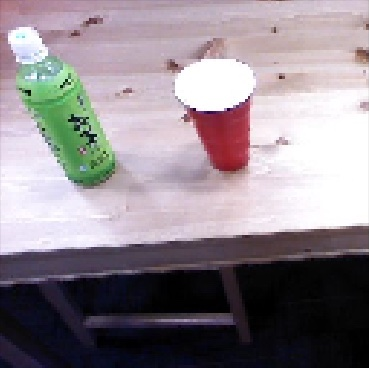
\includegraphics[width=0.31\linewidth]{figures/sim2real/rgb_kitchen_table.jpg}
%     \hfill
%     %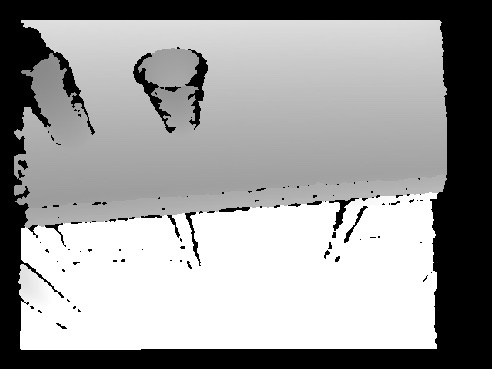
\includegraphics[width=0.31\linewidth]{figures/sim2real/d_kitchen_table.jpg}
%     %\hfill
%     %\includegraphics[width=0.31\linewidth]{example-image-c}
%     \\\vspace{3pt}
%     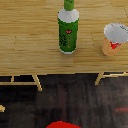
\includegraphics[width=0.31\linewidth]{figures/sim2real/sim_rgb_kitchen_table.jpg}
%     \hfill
%     %\includegraphics[width=0.31\linewidth]{example-image-b}
%     %\hfill
%     %\includegraphics[width=0.31\linewidth]{example-image-c}
%     \\\vspace{10pt}
%     \includegraphics[width=0.31\linewidth]{figures/sim2real/rgb_trash_bin.jpg}
%     \hfill
%     %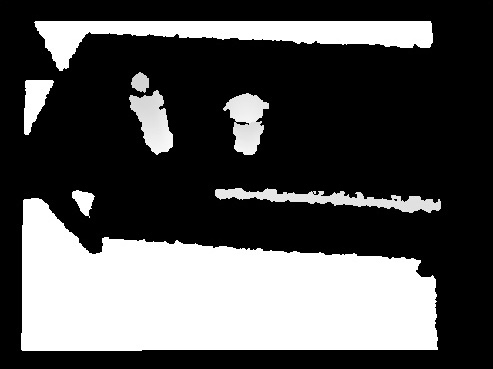
\includegraphics[width=0.31\linewidth]{figures/sim2real/d_coffee_table.jpg}
%     %\hfill
%     %\includegraphics[width=0.31\linewidth]{example-image-c}
%     \\\vspace{3pt}
%     \includegraphics[width=0.31\linewidth]{figures/sim2real/sim_rgb_trash_bin.jpg}
%     \hfill
%     %\includegraphics[width=0.31\linewidth]{example-image-b}
%     %\hfill
%     %\includegraphics[width=0.31\linewidth]{example-image-c}
% %    \caption{\textbf{Comparison between simulated and real sensor signals.} From left to right: RGB, Depth and Lidar signals in simulation (first and third rows) and from the real-world sensors (second and third rows) in two different locations of the \texttt{mockup\_apt} scene (location 1: first two rows, location 2: last two rows). Apart from some unmodeled sources of noise in the real-sensors, we observe a high realism in the signals generated in \simulator.}
%     \caption{\textbf{Comparison between simulated and real sensor signals.} RGB signals in simulation (first and third rows) and from the real-world sensors (second and third rows) in two different locations of the \texttt{mockup\_apt} scene (location 1: first two rows, location 2: last two rows). Apart from some unmodeled sources of noise in the real-sensors, we observe a high realism in the signals generated in \simulator.}
%     \label{fig:simrealsensors}
% \end{figure}

\subsection{Further Characterization of the Sim-Real Gap}

\revision{We performed additional experiments to characterize the gap between simulation and the real world. In our experiments, we moved the robot to different locations in the \texttt{mockup\_apt} scene and collected real sensor signals: RGB images, depth maps, and LiDAR measurements. We then moved the robot in simulation to the same locations and collected virtual sensor signals. Some of the images are depicted in Fig.~\ref{fig:simrealsensors}. We observe that, thanks to our highly realistic models, \simulator provides high-fidelity sensor signals that approximate the real-world ones. However, some of the sources of noise in the real sensors are not modeled currently in \simulator, contributing to a sim-real gap, e.g., the poor dynamic range of the RGB camera, or the ``shadow'' effects in depth maps due to the projected light mechanism. This analysis indicates possible avenues to further close the sensor gap between simulation and the real world, e.g., by including sensor noise models in \simulator or by leveraging sim-to-real techniques (e.g., domain randomization, system identification).}

\subsection{Additional Experiments}
\revision{
In addition to \rlprimhist, we also evaluated \rlvmc and \rlprimhist in the real world and observed a similar trend of performance in the real world as in simulation: \rlvmc < \rlprim < \rlprimhist. \rlvmc still achieves zero success because of sparse reward and exploration difficulty during training. \rlprim has worse performance than \rlprimhist: on average, the robot with \rlprimhist successfully places 0.64 cups/bottles, whereas the one with \rlprim places 0. Qualitatively, \rlprim tends to get stuck in a repetitive action loop because the agent is unaware of its action history. This preliminary result offers us some confidence that \simulator can be a reliable test bed for future sim-to-real robotics research.
}
\begin{figure}[h!]
    \centering
    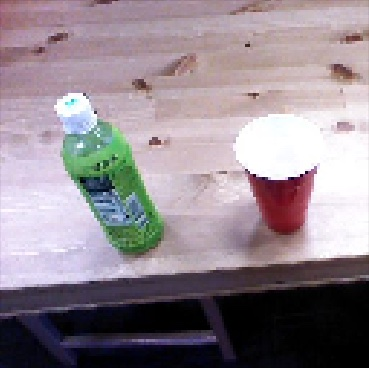
\includegraphics[width=0.31\linewidth]{figures/sim2real/rgb_real_kitchen_table.jpg}
    \hfill
    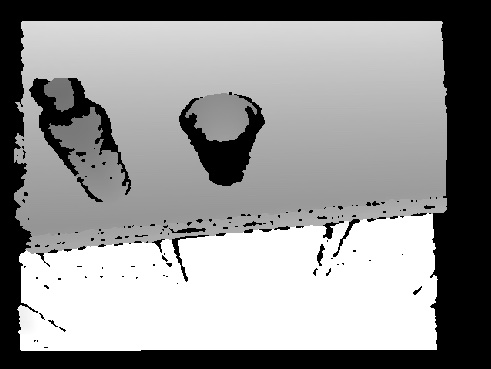
\includegraphics[width=0.31\linewidth]{figures/sim2real/depth_real_kitchen_table.jpg}
    \hfill
    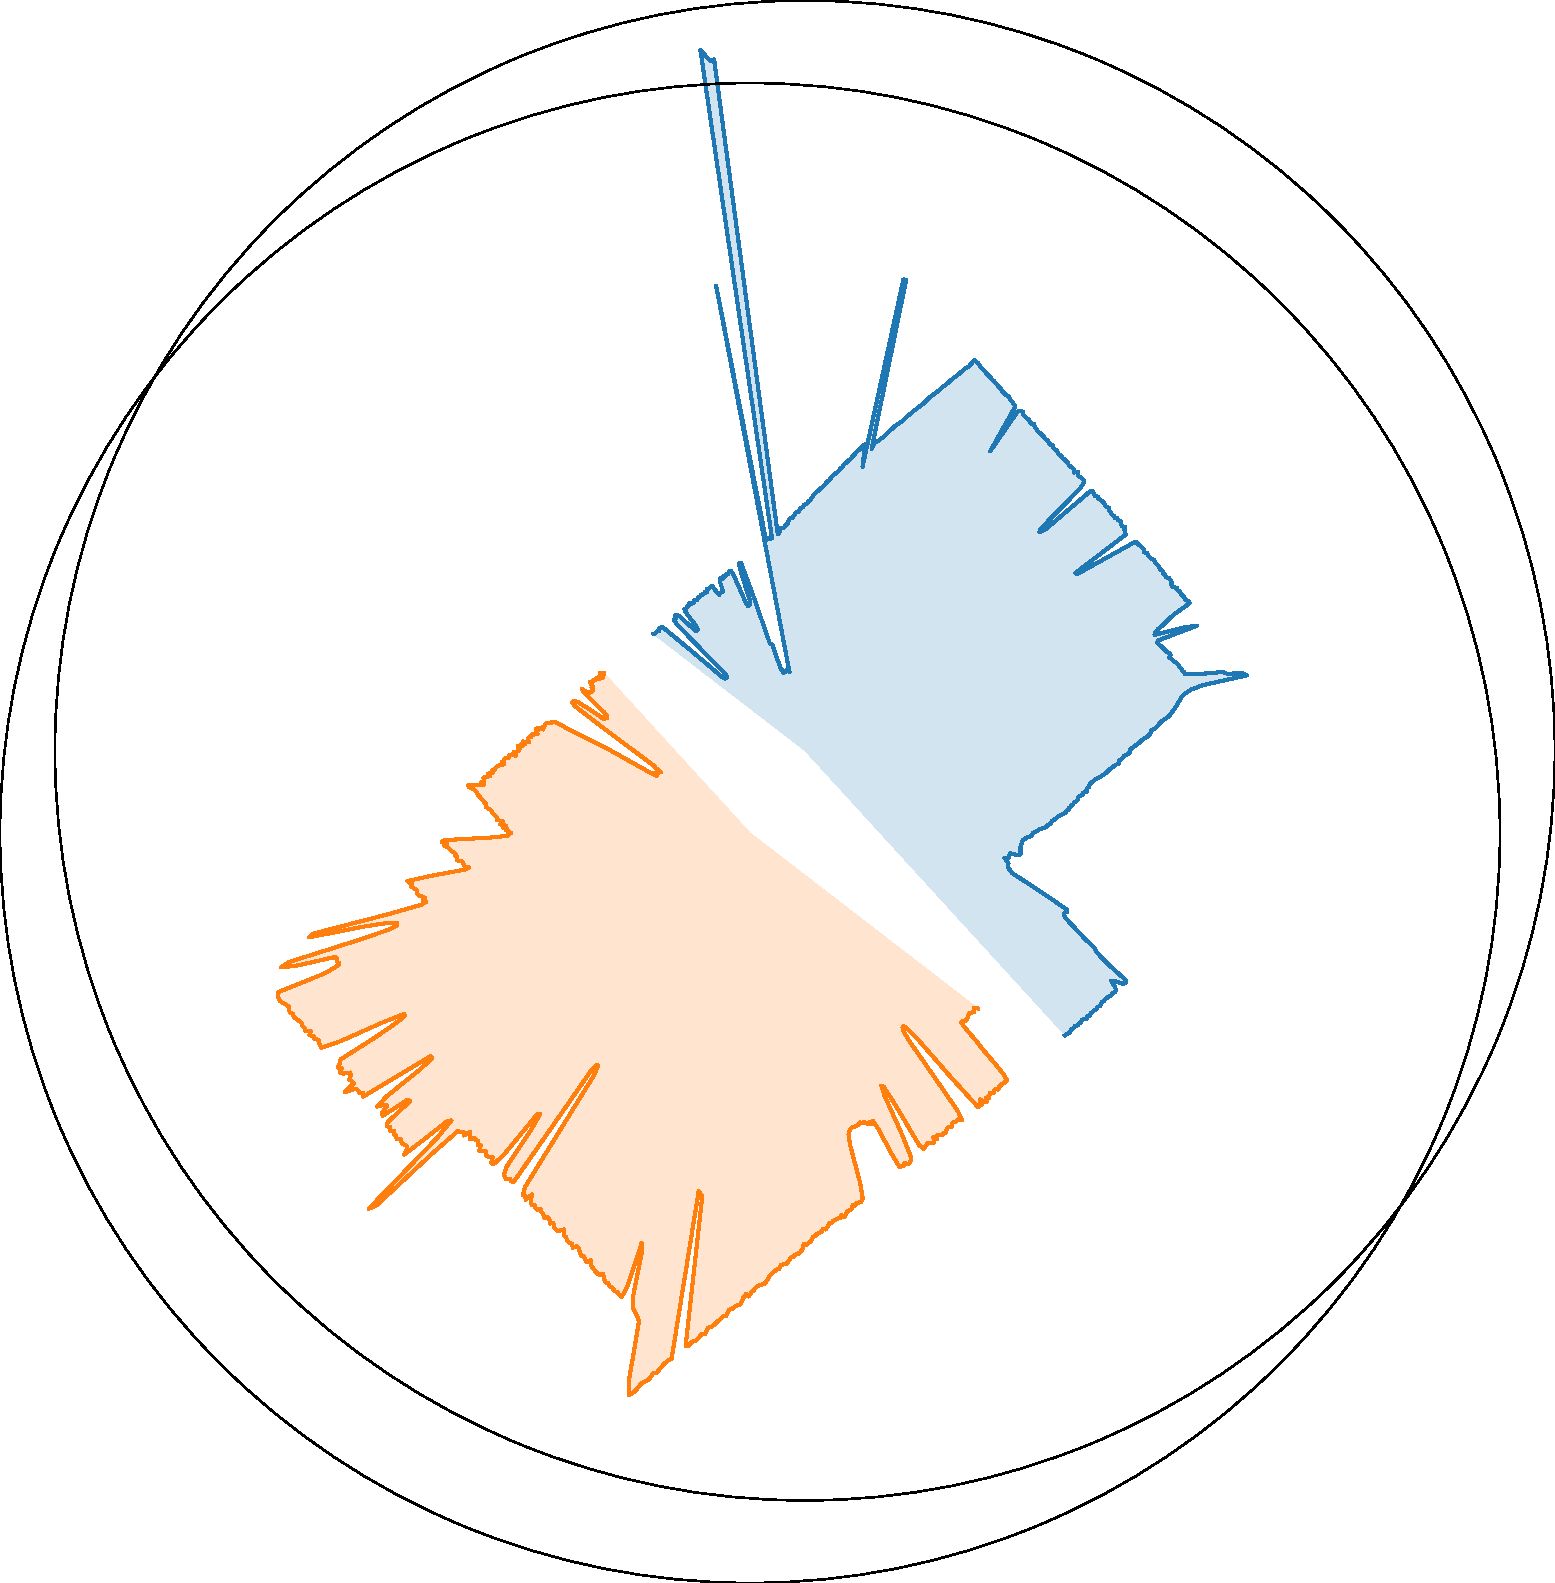
\includegraphics[width=0.31\linewidth]{figures/sim2real/lidar_real_kitchen_table}
    \\\vspace{3pt}
    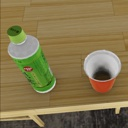
\includegraphics[width=0.31\linewidth]{figures/sim2real/rgb_sim_kitchen_table.jpg}
    \hfill
    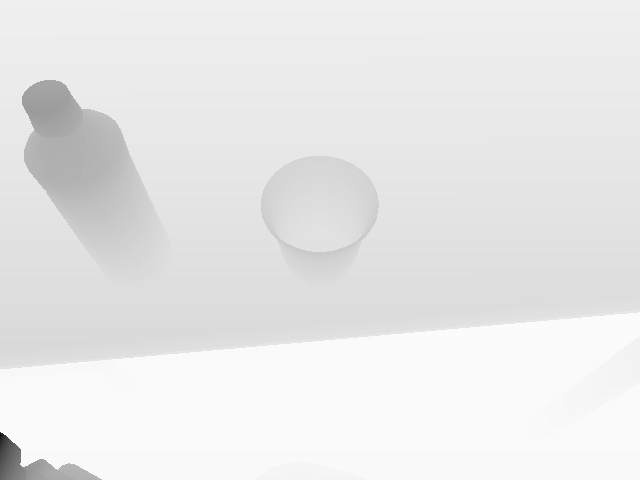
\includegraphics[width=0.31\linewidth]{figures/sim2real/depth_sim_kitchen_table.jpg}
    \hfill
    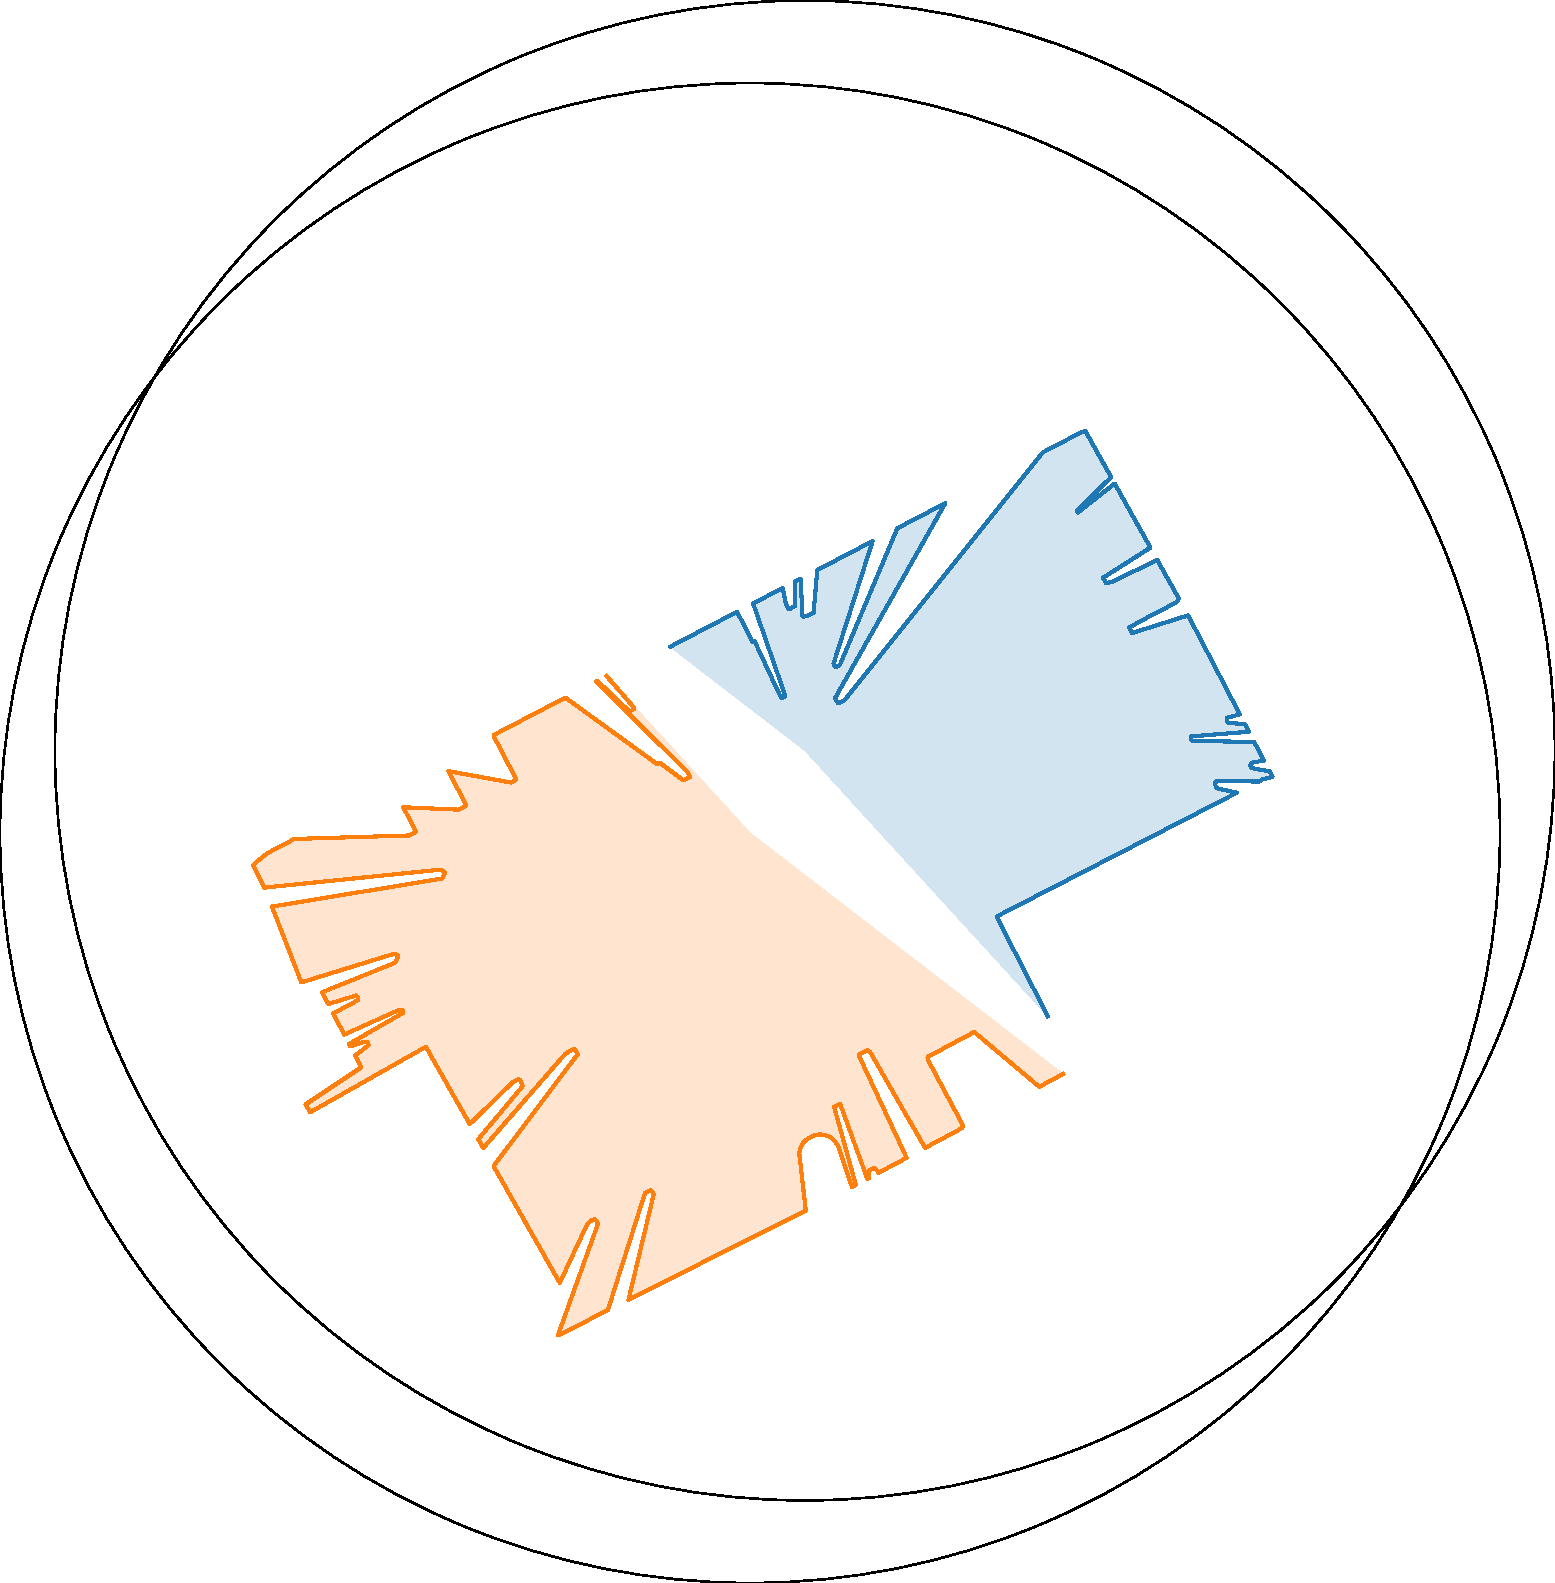
\includegraphics[width=0.31\linewidth]{figures/sim2real/lidar_sim_kitchen_table}
    \\\vspace{10pt}
    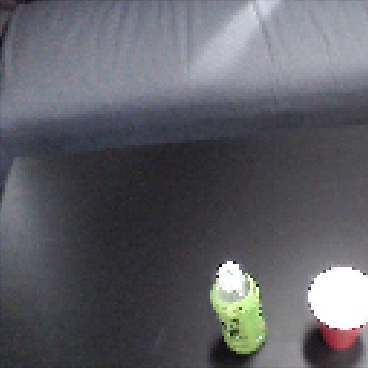
\includegraphics[width=0.31\linewidth]{figures/sim2real/rgb_real_coffee_table}
    \hfill
    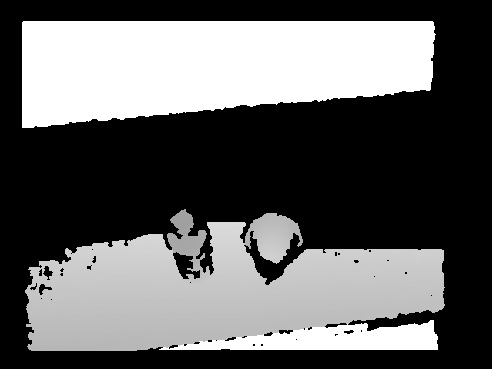
\includegraphics[width=0.31\linewidth]{figures/sim2real/depth_real_coffee_table}
    \hfill
    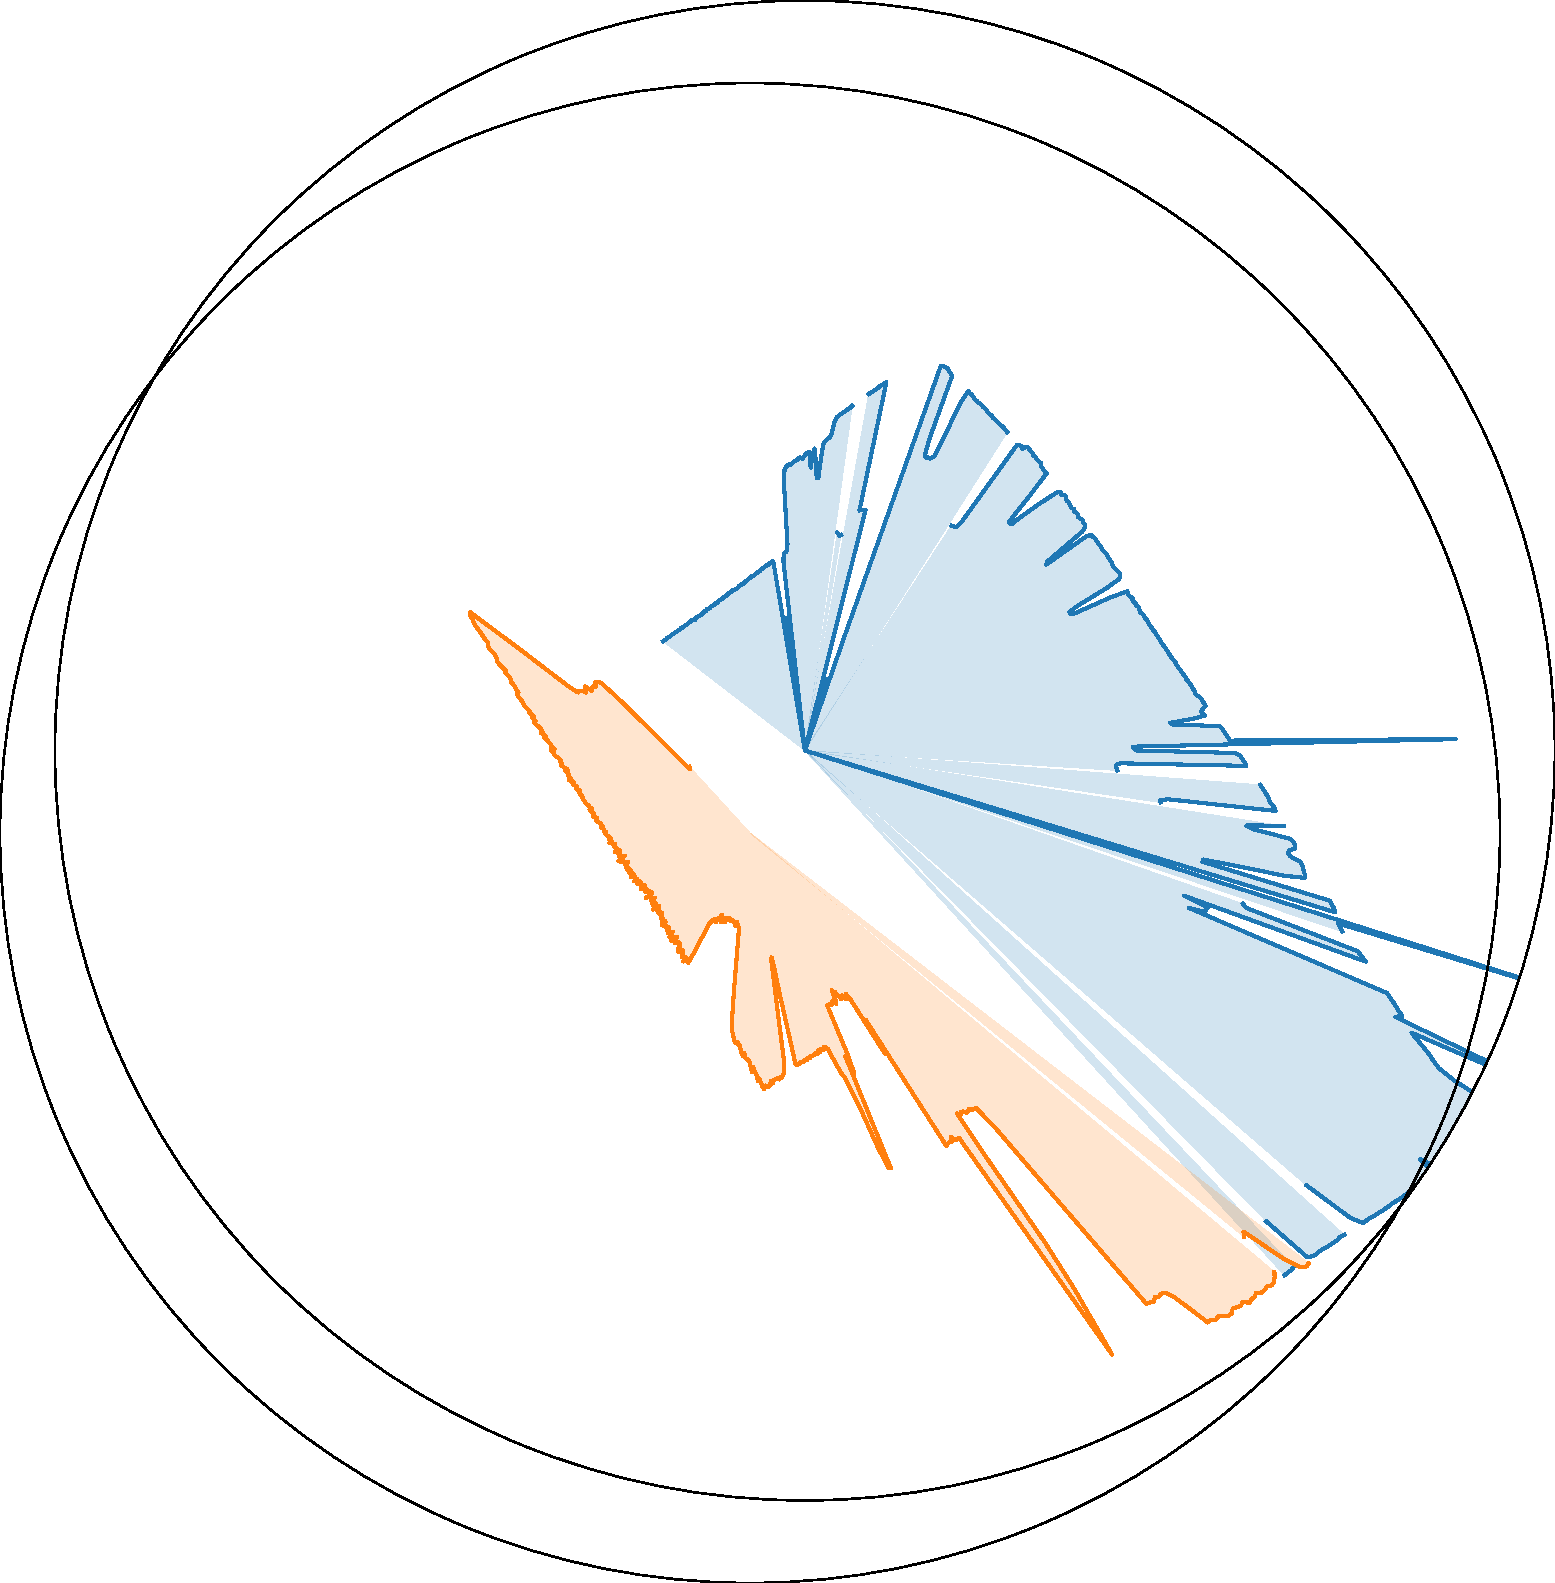
\includegraphics[width=0.31\linewidth]{figures/sim2real/lidar_real_coffee_table}
    \\\vspace{3pt}
    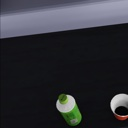
\includegraphics[width=0.31\linewidth]{figures/sim2real/rgb_sim_coffee_table.jpg}
    \hfill
    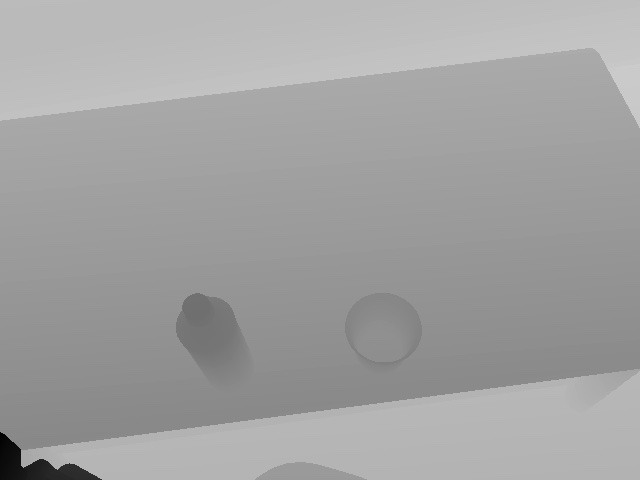
\includegraphics[width=0.31\linewidth]{figures/sim2real/depth_sim_coffee_table.jpg}
    \hfill
    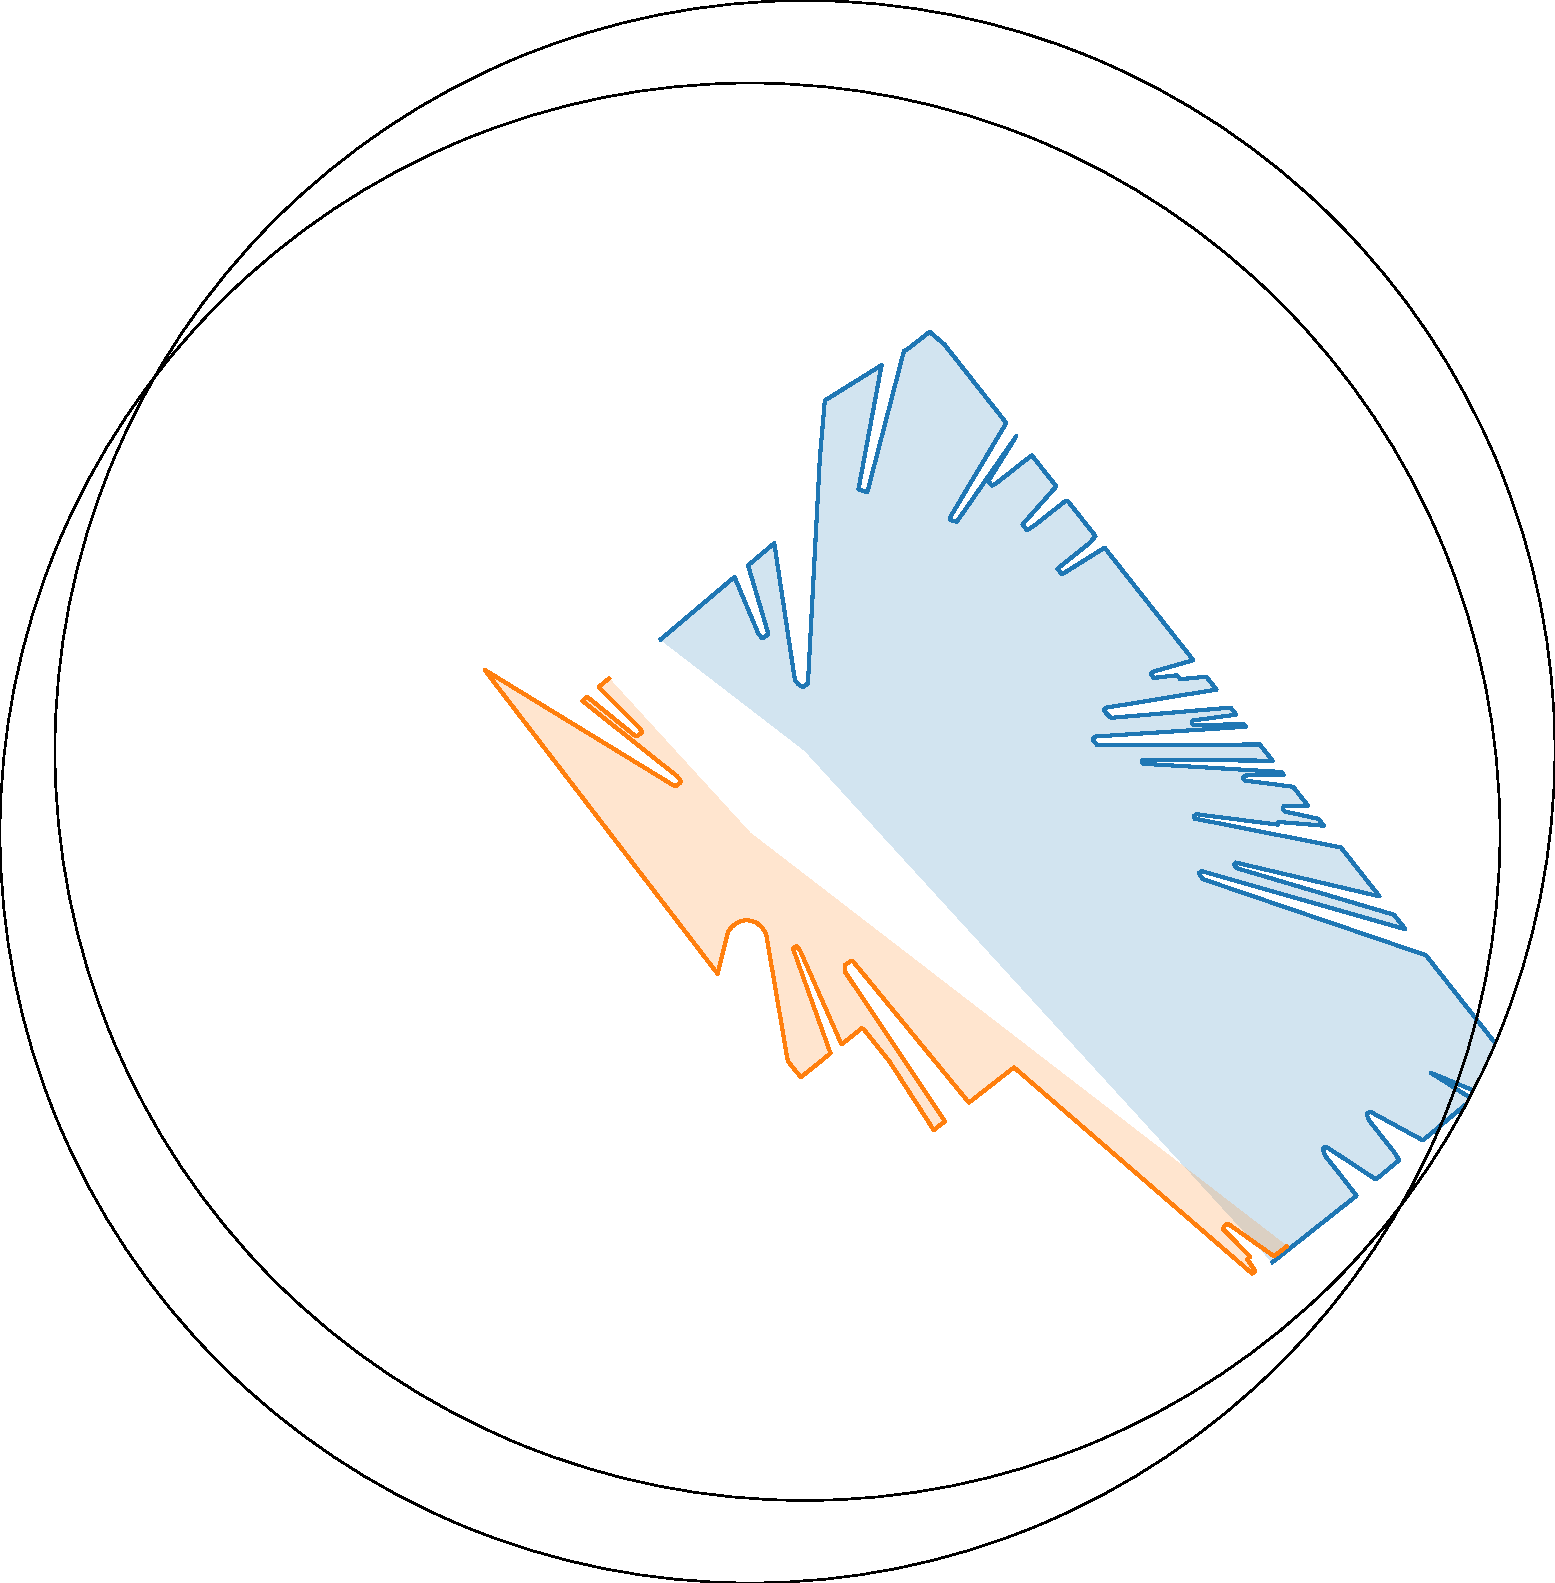
\includegraphics[width=0.31\linewidth]{figures/sim2real/lidar_sim_coffee_table}
    %    \caption{\textbf{Comparison between simulated and real sensor signals.} From left to right: RGB, Depth and Lidar signals in simulation (first and third rows) and from the real-world sensors (second and third rows) in two different locations of the \texttt{mockup\_apt} scene (location 1: first two rows, location 2: last two rows). Apart from some unmodeled sources of noise in the real-sensors, we observe a high realism in the signals generated in \simulator.}
    \caption{\revision{\textbf{Comparison between real and simulated sensor signals.} RGB, Depth and LiDAR signals from the real-world sensors (first and third rows) and from the simulated sensors (second and fourth rows) at two different locations of the \texttt{mockup\_apt} scene (location 1: first two rows, location 2: last two rows). We observed a smaller sensor sim-real gap for LiDAR than for RGB and Depth: RGB is heavily influenced by lighting conditions and camera settings while Depth has difficulty in capturing reflective surfaces.}}
    \label{fig:simrealsensors}
\end{figure}